\documentclass[botnum,fleqn,final]{unmeethesis}

% Set Title and Author
\newcommand{\mytitle}{Information Protection in Content-centric Networks}
\newcommand{\myauthor}{Christopher C. Lamb}


\usepackage[latin1]{inputenc}
\usepackage{amsmath}
\usepackage{amsfonts}
\usepackage{amssymb}
\usepackage{graphicx}
\usepackage{epsfig}
\usepackage{booktabs}
\usepackage{listings}
\usepackage{courier}
\usepackage{multirow}
\usepackage{color}
\usepackage{framed}
\usepackage{lipsum}

% Font settings:
\usepackage[T1]{fontenc}
%\usepackage{mathpazo}
\usepackage{mathptmx}
\usepackage[scaled]{helvet}
\usepackage{courier}
\normalfont

% User microtype package to get some nicer font details
% http://www.ctan.org/tex-archive/macros/latex/contrib/microtype
\usepackage{microtype}

% Other packages
\usepackage{graphicx} % ability to include graphics
\usepackage[pdftex]{hyperref} % hyperrefs inside of PDF
\hypersetup{colorlinks,
            citecolor=black,
            filecolor=black,
            linkcolor=black,
            urlcolor=black,
            pdftitle={\mytitle},
            pdfauthor={\myauthor}}

% Use hyperref package to allow hyperlinks inside of 
% the PDF document and PDF metadata
% http://en.wikibooks.org/wiki/LaTeX/Hyperlinks
\usepackage[pdftex]{hyperref}
\hypersetup{
    %bookmarks=true,          % show bookmarks bar?
    unicode=false,           % non-Latin characters in Acrobat’s bookmarks
    pdftoolbar=true,         % show Acrobat’s toolbar?
    pdfmenubar=true,         % show Acrobat’s menu?
    pdffitwindow=false,      % window fit to page when opened
    pdfstartview={FitH},     % fits the width of the page to the window
    pdftitle={\mytitle},     % title
    pdfauthor={\myauthor},   % author
    pdfsubject={\mytitle},   % subject of the document
    pdfcreator={\myauthor},  % creator of the document
    pdfproducer={\myauthor}, % producer of the document
    colorlinks=true,         % false: boxed links; true: colored links
    linkcolor=black,         % color of internal links
    citecolor=black,         % color of links to bibliography
    filecolor=black,         % color of file links
    urlcolor=blue            % color of external links
}


\graphicspath{{./images/}}
 
\lstset{
	language=IDL,
	basicstyle=\scriptsize\ttfamily, 
	numbers=left,    
	numberstyle=\tiny,
	stepnumber=1,
	numbersep=5pt,
	tabsize=2,
	extendedchars=true,        
	breaklines=true,            
	keywordstyle=\color{red},
	frame=b,         
	stringstyle=\color{white}\ttfamily,
	showspaces=false,
	showtabs=false,
	xleftmargin=17pt,
	framexleftmargin=17pt,
	framexrightmargin=5pt,
	framexbottommargin=4pt,
	showstringspaces=false      
}
 
\usepackage{caption}
\DeclareCaptionFont{white}{\color{white}}
\DeclareCaptionFormat{listing}{\colorbox[cmyk]{0.43, 0.35, 0.35,0.01}{\parbox{\textwidth}{\hspace{15pt}#1#2#3}}}
\captionsetup[lstlisting]{format=listing,labelfont=white,textfont=white, singlelinecheck=false, margin=0pt, font={bf,footnotesize}}

\begin{document}

\frontmatter

\title{\mytitle}
\author{\myauthor}

\degreesubject{Ph.D., Computer Engineering}

\degree{Doctor of Philosophy \\ Computer Engineering}

\documenttype{Dissertation}

\previousdegrees{B.S., Mechanical Engineering, New Mexico State University, 1994 \\
                 M.S., Computer Science, University of New Mexico, 2002}

\date{\today}

\maketitle

\makecopyright

\begin{dedication}
This dissertation is dedicated first and foremost to my wife, who dealt with me, bills, kept our children fed and otherwise kept a roof over my head while I was preoccupied with writing this dissertation.  She took care of everything while working full time in Santa Fe and enabling my higher education addiction.  I could never have accomplished this without her support, love, and encouragement.  She was key in keeping me on some kind of schedule to finish.  Without her gentle reminders regarding the importance of actually {\bf completing} my dissertation, I would likely be submitting this some time in 2014.

This is dedicated to you Missy.
\end{dedication}

\begin{acknowledgments}
   \vspace{1.1in}
I would like to thank my advisor, Professor Greg Heileman, for reading and re-reading my papers and dissertation, and guiding my research.  Truly widely educated with a deep understanding of an astounding number of fields, his guidance and suggestions were invaluable in helping me craft this dissertation.

Thanks to my committee for sitting through my defense, reading this dissertation, and supporting me as well as the larger computer science  and computer engineering disciplines at the University of New Mexico (UNM).  We indeed have world-class academics here at UNM, and I was so very lucky to have some of them working with me, teaching me, and helping me with my research over the (many) years.
   
I would also like to thank everyone in the Informatics Lab.  Their feedback, support, and encouragement was so very helpful in my completion of this dissertation.  Especially Pramod Jamkhedkar, my long time collaborator, and Sinan al-Saffar.  It's especially inspiring when you see someone you work with actually complete a Ph.D program.
\end{acknowledgments}

\maketitleabstract

\begin{abstract}
Information-centric networks have distinct advantages with regard to securing sensitive content as a result of their new approaches to managing data in potential future internet architectures.  These kinds of systems, because of their data-centric perspective, provide the opportunity to embed  policy-centric content management components that can address looming problems in information distribution that both companies and federal agencies are beginning to face with respect to sensitive content.  This work addresses the current state of the art in both these kinds of cross-domain systems and information-centric networking in general.  It then covers other related work, outlining why information-centric networks are more powerful with regard to usage management.  Then, it introduces a taxonomy of types of policy-centric usage managed information-centric network systems and an associated methodology for evaluating the individual taxonomic elements.  It finally delves into experimental evaluation of the various defined architectural options and presents results of comparing experimental evaluation with anticipated outcomes. This work is the end result of four conference papers (IEEE Cloud 2011, ACM DRM 2011, IEEE SoSE '11, and IEEE Cloud 2012), one invited talk (DoDIS 2012), and research performed using this system is currently submitted to two journals for publication (IJ-Closer and Dynamic Work).
\end{abstract}

\tableofcontents
\listoffigures
\listoftables

\begin{glossary}{UHR}
\item[CCN] Content-Centric Network
\item[content network] A network used to store information in which a single query to a contained content node will propagate that query to other systems until a suitable response is found.
\item[content node] A single system in a content network.
\item[content router] An node in a content network that routes queries to child nodes.  Content routers do not contain data, but just route queries.
\item[context] The environment in which a resource is used by a subject.
\item[context manager] A component that manages information associated with a context.
\item[cross domain] Actions that span two or more domains.
\item[cross domain solution] A product that facilitates interoperability between two domains.
\item[DoD] United States Department of Defense
\item[DONA] Data-Oriented Network Architecture
\item[domain (security domain)] A group of systems designed to handle certain specific types of information.
\item[domain ontology] An ontology of data from a specific domain.
\item[enclave] A subset of systems within a domain.
\item[filter] A component generally in a guard that examines a set of data and reacts specific elements of that set according to predetermined rules.
\item[guard] A system between two domains that validates information crossing from one domain to the other as appropriate for storage in the destination domain.
\item[hierarchical content network] A content network organized in a strict hierarchy.
\item[ICN] Information-Centric Network
\item[NetInf] Network of Information
\item[non-hierarchical content network] A content network that is not organized hierarchically.  An example would be a peer-to-peer system.
\item[ontology manager] A component that manages and unifies domain ontologies from different domains.
\item[ontology compiler] A component that compiles an RDF/XML ontology into Ruby.
\item[ontological hierarchy] A hierarchy of ontologies.  Generally associated with policy ontologies.
\item[overlay network] A network of nodes that communicate using the application layer of the TCP/IP or OSI network communication models.
\item[policy] A set of rules that determine how associated content can be used.
\item[policy ontology] The ontology of security policy classifiers in a specific domain.
\item[policy set] A set of policies or policy sets.
\item[PSIRP] Publish-Subscribe Internet Routing Project
\item[resource] Content that is managed from a usage perspective.
\item[rules] A specific description of how a resource can be used.
\item[smashup] A secure mashup application.
\item[subject] An actor that uses a resource.
\item[UCDMO] Unified Cross Domain Management Office
\item[usage management] Managing all aspects of use of an item.
\item[usage management mechanism] A component that manages the use of a resource.
\item[XML] eXtensible Markup Language
\end{glossary}

\mainmatter

\chapter{Introduction}
Current enterprise computing systems are facing a troubling future.  As things stand today, they are too expensive, unreliable, and information dissemination procedures are just too slow.  Current approaches to partitioning information in cross-domain scenarios are simply unable to migrate to cloud environments because of reliance on control of physical hardware to enforce information separation.  The current approach of controlling information by controlling the underlying physical network, the traditional approach to securing information, does not scale into shared datacenters ~\cite{RedBook}.  This leaves large government and commercial organizations concerned with avoiding the exposure of sensitive data in a very uncomfortable position, where they cannot continue doing what they have done, and cannot migrate to what everyone else is doing.

Generally, systems handling sensitive information still do not use current commercial resources as well as they could and use costly data partitioning schemes.  Most of these kinds of systems are managed in house by the enterprise itself rather than exploiting lower cost cloud-enabled services.  Furthermore, many of these systems have large maintenance loads imposed on them as a result of internal infrastructural requirements like data and database management or systems administration.  In many cases networks containing sensitive data are separated from other internal networks to enhance data security at the expense of productivity, leading to decreased working efficiencies and increased costs.

These kinds of large distributed systems suffer from a lack of stability and reliability as a direct result of their inflated provisioning and support costs.  Simply put, the large cost and effort burden of these systems precludes the ability to implement the appropriate redundancy and fault tolerance in any but the absolutely most critical systems ~\cite{Tallon:2010:UDI:1735223.1735253}.  Justifying the costs associated with standard reliability practices like diverse entry or geographically separated hot spares is more and more difficult to do unless forced by draconian legal policy or similarly dire business conditions.

Finally, the length of time between when a sensitive document or other type of data artifact is requested and when it can be delivered to a requester with acceptable need to view that artifact is prohibitively long.  These kinds of sensitive artifacts, usually maintained on partitioned networks or systems, require large amounts of review by specially trained reviewers prior to release to data requesters.  In cases where acquisition of this data is under hard time constraints like sudden market shifts or other unexpected conditional changes this long review time can result in consequences ranging from financial losses to loss of life.

Federal, military, and healthcare computer systems are prime examples of these kinds of problematic distributed systems, and demonstrate the difficulty inherent in implementing new technical solutions.  They, like other similar systems, need to be re-imagined to take advantage of radical market shifts in computational provisioning.  New approaches to networking and information management present possible solutions to these kinds of problems by providing distributed information-centric approaches to data management and transfer ~\cite{proposal:info-sharing-strategy}.

Current policy-centric systems are being forced to move to cloud environments and incorporate much more open systems.  Some of these environments will be private or hybrid cloud systems, where private clouds are infrastructure that is completely run and operated by a single organization for use and provisioning and hybrid clouds are combinations of private and public cloud systems.  Driven by both cost savings and efficiency requirements, this migration will result in a loss of direct control of computing resources by involved organizations as they attempt to exploit economies of scale and utility computing.

Robust usage management will become an even more important issue in these environments.  Federal organizations poised to benefit from this migration include agencies like the United States National Security Agency (NSA) and the United States Department of Defense (DoD), both of whom have large installed bases of compartmentalized and classified data.  The DoD realizes the scope of this effort, understanding that such technical change must incorporate effectively sharing needed data with other federal agencies, foreign governments, and international organizations ~\cite{proposal:info-sharing-strategy}.  Likewise, the NSA is focused on using cloud-centric systems to facilitate information dissemination and sharing ~\cite{proposal:nsa-cloud}.

Cloud systems certainly exhibit economic incentives for use, providing cost savings and flexibility, but they also have distinct disadvantages as well ~\cite{proposal:privacy-security-trust-cloud}.  How to address these issues is an open research question.  Organizations ranging from cloud service providers to the military are exploring how to engineer solutions to these problems, and to more clearly understand the trade-offs required between selected system architectures ~\cite{proposal:assured-info-sharing}.  The problems themselves are wide ranging, appearing in a variety of different systems.  Military and other government systems are clearly impacted by these kinds of trust and security issues, and they also have clear information sensitivity problems.  This, coupled with the fact that these organizations have been dealing with these issues in one form or another for decades make them very well suited for prototypical implementation and study.

This chapter will cover national and international standards in this area, current solutions in place to address some of these problems, the state of the art in information networks, and other related work.  Organizations have been trying to standardize security approaches since the 1980's, starting with the notorious Orange Book ~\cite{OrangeBook}, and ending with today's NIST cloud standards ~\cite{NIST800:144}.  Information-centric networks are a new approach to information management that promises more efficient content  management and supplies new capabilities for information security. The DoD has been key in some of these efforts, and continues to play such a role today, demonstrated in the state of the art in today's cross-platform solutions.  The second chapter introduces and analyzes a proposed architectural taxonomy to address the information sharing goals held by the DoD through the Unified Cross Domain Management Office (UCDMO), and the third describes in detail the development of this prototypical system, starting with a single-system proof-of-concept and working through the current nation-spanning cloud network.  The final chapter covers specific experimental results and analysis of these techniques from a confidentiality, integrity, and availability perspective.

\section{Confidentiality and Integrity Models}
Current models currently in active use to support information confidentiality and integrity include the Bell-LaPadula model, the Biba model,  the Clark-Wilson model, and the Brewer and Nash model.  Of these, Bell-LaPaudula and Brewer and Nash address information confidentiality, while Biba and Clark-Wilson address information integrity.

Bell-LaPadula was developed in the 1970's to address information confidentiality in the centralized mainframe and minicomputer environments  common in military installations of the day.  It is essentially a mathematical state machine model that establishes rules with respect to how information can flow in stratified environments.  It is established around the {\it Basic Security Theorem}, which essentially states that a system with a secure initial state and only secure transitions is guaranteed to terminate in a secure final state.  It extends this theorem to establish four rules.  The first is the {\it simple security rule}.  The simple security property prohibits reading information from security levels higher than that occupied by the reader.  The next two are the {\it *-property rule} and the {\it strong *-property rule}, which prohibit writing data to any security level less than that of the writer.  The final property is the {\it ds-property}, or {\it Discretionary Security Property}.  The ds-property allows a subject to pass permissions on to other subject's at the initial subject's discretion.  This model also introduces the concepts of {\it dominance relations} and {\it tranquility}.  Dominance relations exist within partially ordered sets of classification levels, where higher classification levels are said to dominate lower levels.  This means that if a subject is cleared to access top secret material, that subject can also access secret and confidential material, as both secret and confidential material is considered to be less sensitive that top secret material.  Tranquility limits object state changes after creation.  Essentially, any object is created at a specific sensitivity level and that sensitivity level does not change with time ~\cite{Bell1973}.

The Brewer and Nash model is currently widely used in the financial services industry.  Also referred to as the Chinese Wall Model, this model changes what subjects can access based on a subject's context.  In this model, information is continually monitored so that no subject is allowed access to an object that may create a conflict of interest or other moral hazard.  More generally, access to objects is dynamically evaluated based on the context of a given subject's previous object accesses. This enforces information confidentiality based on the context of information access ~\cite{Brewer89}.

The Biba model, developed in the late 1970's, addresses information integrity using a layered approach similar to that used by Bell-LaPadula, and was in fact developed to complement Bell-Lapadula's focus on confidentiality.  Bell-LaPadula features a hierarchy of information sensitivity that guides access decisions.  Biba, on the other hand, is based on a hierarchy of information integrity rather than confidentiality.  Biba also has a collection of specific properties that must be adhered to.  The first, the {\it simple integrity axiom}, holds that a subject cannot access an object of a lower integrity level.  The second, the {\it *-integrity axiom}, likewise states that a subject cannot write information to higher integrity level.  The third property, the {\it invocation property}, states that subjects cannot invoke objects at higher integrity levels either ~\cite{Biba1977}.

David Clark and David Wilson presented their integrity model in 1987 to address business information integrity as Biba was thought to be more suitable for military use.  The Clark-Wilson model uses five essential components.  The first, {\it users}, are active subjects requesting access to objects.  The second, {\it transformation procedures}, are operations allowed over objects.  These general operations are any that may change the state of an object, like create, update, and delete operations, as well as simple read access.  Systems are also required to have collections of {\it integrity verification procedures} which validate the state of managed objects.  The object themselves have two distinct flavors, {\it constrained data items} and {\it unconstrained data items}.  Constrained data items are those managed via trusted transformation procedures and monitored via integrity verification procedures.  Unconstrained items can be directly accessed.  Access and management of data items are constrained by a set of nine rules, divided into sets of certification and integrity rules.  In essence, these rules ensure that all constrained data item access is through trusted transformation procedures, and that the trusted procedures ensure that information is maintained in a valid state.  Subjects are limited to sets of trusted transformation procedures expressed by $(subject, procedure, object)$ triples, while unconstrained data items can be accessed without limitation ~\cite{ClaWil87}.






\section{National and International Standards}
Once the Bell-LaPadula and Biba models were in developed and understood, the Department of  started another effort to more clearly categorize the security of information systems and related networks.  This effort cumulated in what is now known as the Rainbow Series of books, specifically the {\it Trusted Computer System Evaluation Criteria}, known as the Orange Book, and the {\it Trusted Network Interpretation}, or Red Book.

The Orange Book addresses security of individual computer systems.  It establishes a taxonomy of security levels at which systems can be classified.  These levels range from systems with minimal security characteristics and stretch to formally verified computer systems.  These levels establish such characteristics as separate administrator accounts, role-based security systems, data labeling, and the recognition of possible covert communications channels ~\cite{OrangeBook}.

The Red Book deals with how networks protect the confidentiality, integrity, and availability of information.  It addresses encryption, digital signatures, flow protection and confidentiality, data confidentiality, and infrastructure protection.  Like the Orange Book, it is a framework established over a set of principles to facilitate network security.  It discusses how subjects and objects need to be controlled and accounted for in computer networks just as they are within individual computer systems ~\cite{RedBook}.

Today, the Rainbow Series has largely been supplanted by the International Organization for Standardization's Common Criteria.  The Rainbow Series was seen as too rigid, and other standards too flexible and difficult to implement, leading to the development of the Common Criteria in 1993.  The Common Criteria are based on Rainbow Series, the Canadian Trusted Computer Product Evaluation Criteria (CTCPEC), and the Information Technology Security Evaluation Criteria (ITSEC).  While the Orange Book examined a system based on a Bell-LaPadula-centric perspective, the Common Criteria evaluates computing systems based on a pre-established protection profile, designed to cover a specific security requirement.  The common criteria also use a taxonomy to classify systems.  This taxonomy has seven levels, again ranging from minimally tested systems that have some assured functionality to formally verified, designed, and tested information systems ~\cite{CommonCriteria}.

Other standards commonly referenced include publications from the National Institute of Standards and Technology, particularly from their 800-series of special publications.  These publications cover everything from cloud computing security ~\cite{NIST800:144} to single computer systems \cite{NIST800:12} to web services \cite{NIST800:95}.
\section{Current Solutions}
\label{section:current-solutions}
The Unified Cross Domain Management Office (UCDMO) supports efforts to develop specific solutions to cross-domain information sharing.  Solution architectures have been presented over the past few years to handle this kind of information management.  The National Security Agency set the standard in this area initially.  In 2009, at a conference sponsored by the UCDMO, Booz Allen Hamilton (BAH) and Raytheon presented alternative notional architectures contrasting with current NSA-influenced approaches ~\cite{proposal:nsa-arch,proposal:gig-arch,proposal:bah-arch,proposal:raytheon-arch}.

The current standard architectural model in place and governed by the UCDMO to deal with these kinds of issues are guard-centric cross domain architectures.  As we will show, the thinking behind these system architectures has remained relatively static over the past 20 years.  New thinking with regard to future internet architectures and usage management provide more powerful approaches to securing information as it flows through dynamic systems.

Current and near-future proposed solutions endorsed by the UCDMO include system architectures assembled by the NSA, Raytheon, and Booz $\mid$  Allen $\mid$  Hamilton (BAH).   The NSA has been active in this area for decades as a logical extension of their role in signals intelligence collection and processing.  Raytheon and BAH have been engaged over the past few years to provide an alternative voice and design approach to these kinds of systems, an effort met with limited success.


\begin{figure}[!t]
\centering
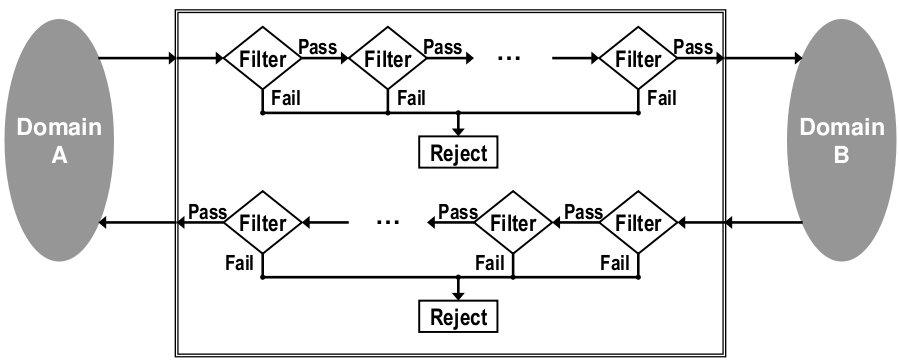
\includegraphics[width=5in]{nsa-legacy-arch}
\caption{NSA Legacy Notional Architecture Model}
\label{fig:model:conceptual-model}
\end{figure}

These cross-domain solutions are intended to enable sensitive information to easily flow both from a higher sensitivity domain to a lower sensitivity domain, and from lower to higher as well.  They generally act over both primary data (say, a document) and metadata over that primary data.

\subsection{NSA, Filtered}
The NSA conducted initial work in this area.  Their standard-setting efforts culminated in a reasonable conceptual system architecture, using groups of filters dedicated to specific delineated tasks to process sensitive information ~\cite{proposal:nsa-arch}. In the scenario portrayed in Figure ~\ref{fig:model:conceptual-model}, \textit{Domain A} could very well be a private cloud managed by the U.S. Air Force, while \textit{Domain B} is a public operational network of some kind shared by coalition partners in a joint operation.

A system user attempts to send a \textit{data package} consisting of a primary document and associated metadata from \textit{Domain A} to \textit{Domain B}.  At some point, that submission reaches a \textit{guard}, which contains at least one \textit{filter chain}.  Each filter chain then contains at least one \textit{filter}.  Individual filters can execute arbitrary actions over a submitted data package and have access to any number of external resources as required.  At any point, a filter can examine the data package and reject it, at which point it will frequently wait for human review.  If a filter does not reject a data package, it passes that package onto the next filter or submits it for delivery to Domain B.

\subsection{NSA, Services}
In recent years, the NSA has extended the legacy system architecture for cross-domain information sharing to exploit service-oriented computing styles ~\cite{proposal:nsa-arch}.  Visualized in Figure ~\ref{fig:model:conceptual-model-services}, this model incorporates more modern conceptual elements and componentry.

Figure ~\ref{fig:model:conceptual-model-services} shows on the left the \textit{Global Information Grid}, or \textit{GIG}.  On the right, the \textit{Distributed Service-oriented Cross Domain Solution}, or \textit{DSCDS}.  The GIG is not a truly open system --- rather, it is a loosely coupled collection of computational services handing data at a variety of levels of sensitivity, federated to provide stakeholders timely access to relevant information ~\cite{proposal:gig-arch}.  The DSCDS is essentially the embodiment of the NSA's cross-domain vision applied to service oriented computing.  This model fuses various technology choices with previous cross-domain thinking.

\begin{figure}[!t]
\centering
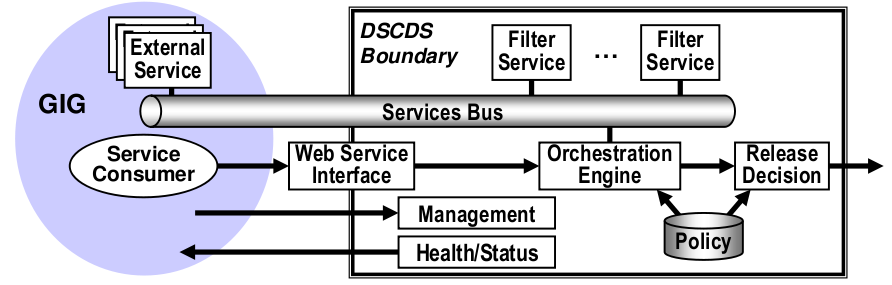
\includegraphics[width=5in]{nsa-arch}
\caption{NSA Service-Oriented Model}
\label{fig:model:conceptual-model-services}
\end{figure}

Indicative of this more modern system design thinking, a variety of services and service consumers are attached to a common service bus within the GIG.  Within the DSCDS, groups of filters are implemented as services inspecting transferred data when moved over the bus.  Finally, all of this interaction is managed by a management interface and controlled by an orchestration engine accessing a centralized group of policies.

Note that here a common policy repository for various types of security metadata over primary data elements has begun to be accessed.

\subsection{Raytheon}
In the past few years, Raytheon has offered a new model for cross domain use influenced by the NSA service-oriented model ~\cite{proposal:raytheon-arch}.  The model in Figure ~\ref{fig:model:conceptual-model-ray} is more grounded in the actual technical environment this kind of solution would be embedded within.  The Non-secure Internet Protocol Router Network (NIPRNet) is one domain, and the Secret Internet Protocol Router Network (SIPRNet) is the other.  Here, NIPRNet is the lower security domain (lowside), and SIPRNet the higher security domain (highside).  This particular view shows the motion of data from the high side (SIPRNet) to the low side (NIPRNet).

\begin{figure}[!t]
\centering
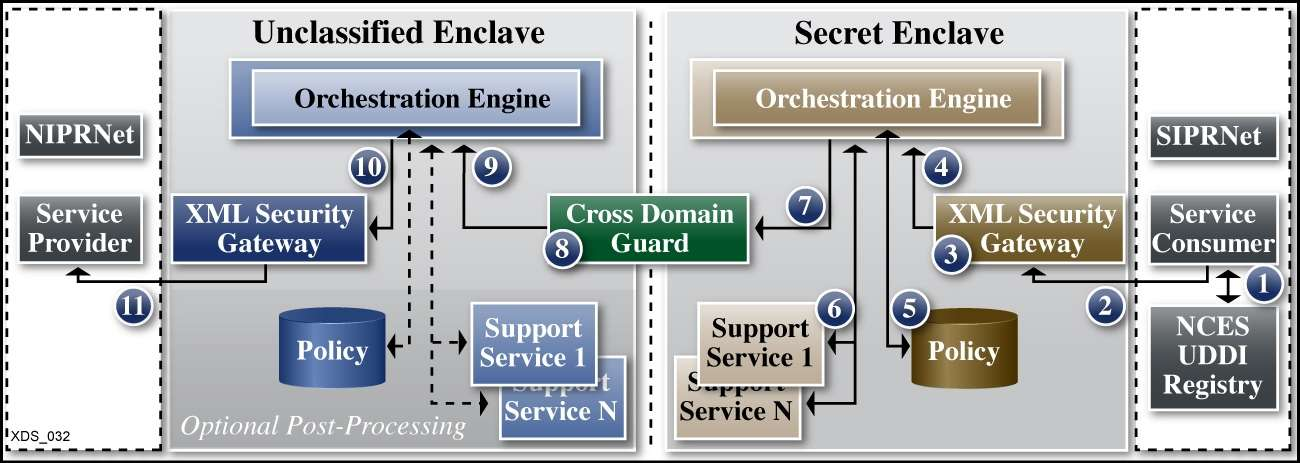
\includegraphics[width=5in]{raytheon-arch}
\caption{Ratheon Model}
\label{fig:model:conceptual-model-ray}
\end{figure}

Here, a data request is submitted from SIPRNet first to the \textit{XML Security Gateway} which calls into the \textit{Orchestration Engine} for policy validation.  The Orchestration Engine then coordinates calls into a \textit{Policy Repository} as well as to a collection of external \textit{Support Services}.  Once rectified against these elements, the request is passed into the \textit{Cross Domain Guard} which routes the request into the \textit{Unclassified Enclave} in NIPRNet.  Here, the request is passed directly through the lowside \textit{XML Security Gateway}, without rectification, onto the \textit{Service Provider}.  The response from the Service Provider is then passed back to the requester via the inverse path.

This model also begins to use a centralized policy repository, just as the NSA Service Model does.  It also uses a single cross domain guard to transfer information from both the highside to the lowside, and vice-versa.

\subsection{Booz $\mid$ Allen $\mid$ Hamilton}
BAH submitted a competing model, also in 2009 ~\cite{proposal:bah-arch}.  In fact, both Raytheon and BAH presented their models under competitive contract to the UCDMO at the same conference, so the domain application is not coincidental.  Figure ~\ref{fig:model:conceptual-model-bah} embodies BAH's thinking with respect to cross domain information management.  It showcases a \textit{Domain A} as a high security domain, and \textit{Domain B} as a low security domain.  Here, dataflow again exists from the highside to the lowside through the cross domain management system.

\begin{figure}[!t]
\centering
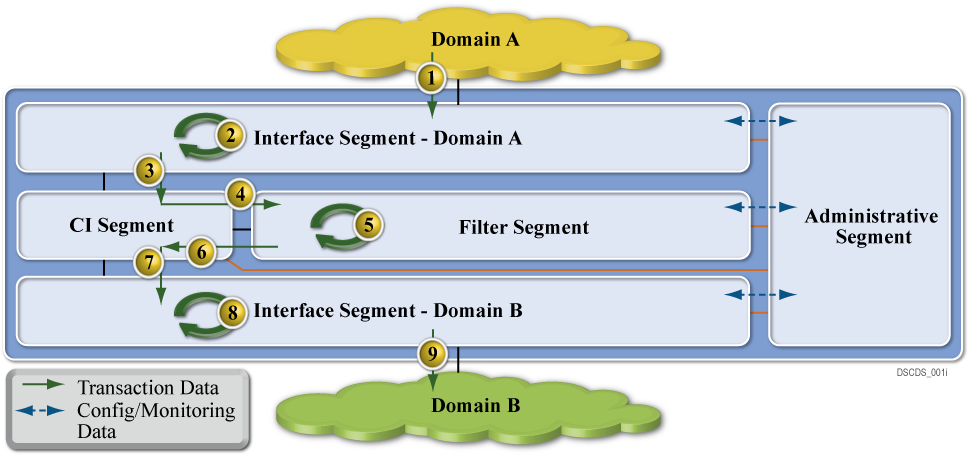
\includegraphics[width=5in]{bah-arch}
\caption{Booz $\mid$ Allen $\mid$ Hamilton Model}
\label{fig:model:conceptual-model-bah}
\end{figure}

While not as detailed as the Raytheon proposal, this does have similar elements.  Here, the data first travels from Domain A into the \textit{Interface Segment for Domain A}, similar to the secret enclave used in the Raytheon model.  From there, it moves into the \textit{CI Segment}, which in turn submits the transferring data into the \textit{Filter Segment}.  From there, the package is moved into the \textit{Interface Segment for Domain B}, and then onto \textit{Domain B}.  The \textit{Administrative Segment} provides management and oversight of the system as a whole.  Note the absence of specific policy-centric elements.  This system is reliant on specific policy-agnostic content filters as well.
\subsubsection*{Shortcomings of Current Systems}
Having reviewed the current state of the art of these kinds of cross domain solutions,  they still have clear similarities, and in fact have not progressed far beyond the initial notions of how these kinds of systems should work.  They still, for example, all use some kind of filter chaining mechanism to evaluate whether a given data item can be moved from a classified to an unclassified network.  Both NSA models used filters explicitly, as did the BAH model.  They all use a single guard as well, a sole point of security and enforcement, providing perimeter data security, but nothing else.  In each of these current system architectures, users are only allowed to exchange one type of information per domain.  The physical instantiations of these models are locked by operational policy to a single classification level limit.  Users cannot, for example, have Top Secret material on a network accredited for Secret material.  Finally, these models violate the end-to-end principle in large service network design, centralizing intelligence rather than pushing that intelligence down to the ends of the system \cite{Blumenthal:2001:RDI:383034.383037}.

\subsubsection*{Characteristics of Future Systems}
Future systems will generally demonstrate decentralized policy management capabilities, infrastructural reuse, the ability to integrate with cloud systems, and security in depth.  Policy management is decentralized and integrated within the fabric of the system.  The system is both more secure and resilient as a result, better able to control information and operate under stressful conditions.  Multi-tenancy can lower costs and increase reliability and is furthermore a common attribute of cloud systems.  An appropriately secured system facilitates integration of computing resources into multi-tenant environments.  The ability to handle multi-tenant environments and to reliably secure both data at rest and data in motion leads to computational environments deployable in cloud systems.  Finally, systems must operate under \textit{all} conditions, including when they are under attack or compromise \cite{proposal:ron-ross}.  Ergo, they must provide protection to sensitive data in depth.

\subsection{Other Related Work}
This work introduces the notion of usage management embedded in a delivery network itself.  It also provides an in-depth analysis of the challenges and principles involved in the design of an open, inter-operable usage management framework that operates over this kind of environment. Besides referencing the material we have covered in depth to portray the current state of the art, the analysis includes application of well-known principles of system design and standards~\cite{BlCl:01,Cl:88,ClWrSoBr:02}, research developments in the areas of usage control~\cite{PaSa:04,JaHeLa:10}, policy languages design principles~\cite{JaHeMa:06}, digital rights management (DRM) systems~\cite{JaHe:09},  and interoperability~\cite{JaHe:04,HeJa:05,KoLaMaMi:04,coral,marlin} towards the development of supporting frameworks.

While a large body of work exists on how overlay networks can use policies for \textit{network} management, very little work has been done on using usage policies for \textit{content} management.  The primary contribution in this area focuses on dividing a given system into specific \textit{security domains} which are governed by individual policies \cite{4457175}.  This system fits into our proposed taxonomy as an $\alpha$-type system as it has domains with single separating guards.

A large body of work currently exists with respect to security in and securing overlay networks.  These kinds of techniques and this area of study is vital to the production development and delivery of overlay systems, but is outside the scope of this work.
\section{Information-centric Networking}
\label{section:information-centric-networking}
Information-centric networking (ICN) is a new approach to internet-scale networks.  In general, it takes extensive advantage of data locality, cache data aggressively, decouple information providers from consumers, and use a content-centric perspective in network design. The overriding goals of this approach include providing higher information availability through better network resilience and implementing systems that more closely reflect today's use, focusing on heterogeneous systems from mobile to static access \cite{6231276}.  Four of the leading projects implementing these ideas are Data-Oriented Network Architecture (DONA) ~\cite{Koponen:2007:DNA:1282427.1282402}, Content-centric Networking (CCN) ~\cite{NDN,CCNx}, the Publish-Subscribe Internet Routing Project (PSIRP) ~\cite{PSIRP}, and the Network for Information (NetInf) ~\cite{NetInf}.  In general these projects and the thinking behind them is motivated by the belief that the current internet is not well suited to the way it is used today and that in order to efficiently support future use the internet needs to be fundamentally re-examined and perhaps re-implemented.

%who what why how % when where
%		
%II. Common Features
%	why they have common features
%	Primitives and design approaches
%		contrast with past internet paradigms
%		current API structural commonalities (use IDL!)
%		how they would work

As expected, given that they are trying to solve similar problems and have taken similar conceptual approaches, the capabilities and features of these projects are similar as well.  To begin with, they all use named data objects as a central abstraction.  In this paradigm, information elements like videos, web pages, databases, and the like are represented by unique names rather than locations.  Current internet systems blur this distinction.  Uniform Resource Locators (URLs) were never designed to be used as content names, for example.  They are content addresses, describing the server and port on which content resides, the protocol to use to retrieve the content, and the specific location of that content on the identified server ~\cite{rfc3986}.  That said, they are still commonly used to name content, particularly in caching systems ~\cite{rfc2616} and content distribution networks ~\cite{Nygren:2010:ANP:1842733.1842736}.  The names of these data objects, since they have unique relationships to content, are tightly bound to the content they represent.  These names need to exhibit strong name-data integrity, so that the name can be trusted to refer to specific content, and the object retrieved must be verifiably authentic.  They have very similar programming interfaces.  These interfaces are built around acquiring and routing specific data objects from providers to consumers rather than forwarding bits from one system to another ~\cite{rfc791,rfc793}.  As a result, operations are oriented more toward registering interest in a named data object in some way, either through a specific object request or subscription, and the resulting delivery of that object ~\cite{6231276}.  ICN systems route information in similar ways as well, depending on the specific naming topology used as well.  Some ICN systems use name resolution services to bind specific objects to names ~\cite{4698847} while others use direct routing schemes to multiple hosts ~\cite{Ghodsi:2011:NCA:2018584.2018586}.  Finally, data objects are frequently cached on devices, both on edge devices and in-network.  These caches are generic and usable by any other services distributed throughout the network ~\cite{6231276}.



		
%III. Differentiating Features
%	what are they
%	why are the different
%	what capabilities to the differences give us
%
%IV. Current Projects (just text, paragraph per, ref projects and survey paper)
%
%V. Conclude
%	impact if successful
%	what else? motivate importance of this work!
	
\section{Other Related Work}
This work introduces the notion of usage management embedded in a delivery network itself.  It also provides an in-depth analysis of the challenges and principles involved in the design of an open, inter-operable usage management framework that operates over this kind of environment. Besides referencing the material covered in depth to portray the current state of the art, the analysis includes application of well-known principles of system design and standards~~\cite{Blumenthal:2001:RDI:383034.383037,Clark:1995:DPD:205447.205458,ClWrSoBr:02}, research developments in the areas of usage control~~\cite{PaSa:04,JaHeLa:10}, policy languages design principles~~\cite{JaHeMa:06}, digital rights management (DRM) systems~~\cite{JaHe:09},  and interoperability~~\cite{JaHe:04,HeJa:05,KoLaMaMi:04,coral,marlin} towards the development of supporting frameworks.

While a large body of work exists on how overlay networks can use policies for \textit{network} management, very little work has been done on using usage policies for \textit{content} management.  The primary contribution in this area focuses on dividing a given system into specific \textit{security domains} which are governed by individual policies ~\cite{4457175}.  This system fits into this proposed taxonomy as an $\alpha$-type system as it has domains with single separating guards.

A large body of work currently exists with respect to security in and over overlay networks.  These kinds of techniques and this area of study is vital to the production development and delivery of overlay systems, but is outside the scope of this work.
\section{Applying Usage Management}
The current state of usage management and control in distributed systems has been addressed from a variety of perspectives, ranging from the United States government to the international community.  Today, organizations have robust models, international standards, and technological approaches that can all be brought to bear on their information management problems.  Information-centric networks present an unaddressed opportunity to bring these standards and theoretical solutions together into a new type of systems providing unique and more powerful information management capabilities.  The next chapter addresses specifically how to migrate these capabilities into information-centric networks and the characteristics of those networks once they have these capabilities.

\chapter{Usage Management in Information-centric Networks}
With the stage set with respect to current technologies and approaches, this chapter will delve into how to apply these techniques in a network setting.  This chapter first addresses specifically why a content-centered perspective when networking information systems provides capabilities that are rendered very difficult to address via traditional, packetized networks.  It then covers the characteristics of information networks that protect information, based on perspectives from industry, government, and the military, describes a taxonomy for approaching ubiquitous network information management, and then analyzes the proposed taxonomy.

\label{section:capabilities}
When it comes to managing the usage of information resources,  information-centric networks provide capabilities that traditional packetized networks cannot.  The basic structure of packet networks facilitates simple and efficient data transfer, but is fundamentally based on certain design assumptions that render network-centric usage management difficult at best and impossible at worst ~\cite{Cl:88,SaReCl:84}.  Information-centric networks, taking a very different approach to network design, are much more amenable to embedded content control based on their different design principles ~\ref{section:information-centric-networking}.

Current packet-based systems share three underlying design principles.  Strict layering, in which upper layers only use services that exist in lower layers which in turn have no knowledge of upper layers, end-to-end arguments governing service placement, and limited runtime packet sizes.  All three of these increase the difficulty in applying control over information trasmitted through networks.

In internet systems, switching and routing traditionally occur in the lower layers of the OSI model ~\cite{Tanenbaum:1985:CN:536716}.  These decisions are made based on a priori knowledge of a given network topology, by manual or programmatic configuration ~\cite{proposal:openflow} and are not impacted by transmitted content except in very high-end systems ~\cite{cisco-6500}.  In fact, access to application content occurs at much higher levels ~\cite{Tanenbaum:1985:CN:536716}.  As a result of strict service layering, the information needed to make content-sensitive routing decisions is simply not available without breaking layer encapsulation on these kinds of devices.  Granted, Vendors do provide switches that examine application-level traffic ~\cite{cisco-6500}.  These intelligent switches are expensive however and as a result are only feasible for large ISPs to deploy. 

End-to-end arguments dictate where services should be placed in a network.  Services like information distribution control that require access to application layer data should, following these principles, be deployed into the ends of a given network ~\cite{SaReCl:84}.  Admittedly, this does encourage scalable network design, by keeping the core of a network simple, efficient, and fast. It however does not support granular information distribution control based on content rather than topology.  In order to control information flow based on content, internal network nodes must be able to access and evaluate transmitted content.  The fundamental end-to-end principles when applied to this problem would strictly prohibit that kind of content analysis.

Likewise, policies associated with content can be arbitrarily large.  As a result, they can exceed maximum packet sizes defined in packetized networks.  Furthermore, as content-sensitive networks must evaluate defined policies prior to routing content, any policy to be evaluated must be completely downloaded into a router and analyzed for suitability for transmission prior to any packet routing, leading to inevitable bottlenecks as content is queued behind the policy elements.

Content analysis of certain kinds of transmitted artifacts may not be possible without a holistic perspective either.  For example, if I have an XML document transmitted through a network, that document may very well have content in element $n$ which is described in more detail in element $n+2$.  Here, element $n$ and element $n+2$, by themselves, are not sensitive.  When combined however, they are.  When transmitted, these elements would be in separate packets.  For the sake of this argument, assume these packets are built such that element $n$ is in packet $m$, and element $n+2$ is in packet $m+c$, where $c$ is some constant, and that packet $m$ is assembled and transmitted from the source node at some time prior to packet $m+c$.  In this scenario, packet $m$ will be passed through an intervening nodes prior to packet $m+c$.  Even nodes that maintain a history of transmitted content that may be able to determine that information in $m$ is sensitive when combined with information in $m+c$ will be unable to undo the ealier transmission of packet $m$.  In order to cicumvent this problem, nodes would need to hold packet for some time $t$ to check for context.  This may help solve the problem, as related information likely has some kind of intrinsic locality, but nevertheless the size of $c$ can be still be relatively arbitrary.  As a result, the size of $t$ is impossible to set {\it a priori}.  This approach imposes possibly significant performance penalties as well.

Information-centric networks are based on different primitives, as described in Section ~\ref{section:information-centric-networking}.  Specifically, they are based on named data objects with strict name-data integrity, as well as other associated principles.  This different abstraction makes policy evaluation and content binding simpler, as content can be bound either in-line to policy or via specific naming conventions.  In these systems, once content is located by name, it is returned to the requester either via a predefined path mirroring the original request path or a variable response path.  In either case however, all content and associated policy is available at each routing node in that return path, and can be evaluated for suitability of transmission.

As a result of these fundamentaly different underlying models, information-centric networks in the next-generation internet enable usage management capabilities that are very problematic to implement and enforce in current internet architectures without dedicated application-level overlays.
\section{Characteristics}
\label{section:characteristics}
Examining content at each network node or router point can certainly impact performance and by extension availability.  It is also important to establish that this kind of dynamic dispatch will actually guarantee delivery along the most secure path needed.  With respect to delivery, it need to be shown that by selecting optimum paths at given network points the overall selected path will have the appropriate security characteristics outlined by any policy associated with delivered content.

To begin with, imagine in a given aggregate path between two points if local decisions are made with respect to routing based on specific security criteria at interleaving points the path as a whole will adhere to those security criteria.  Essentially, this implies that it is possible to use a greedy algorithm with respect to security and routing and that the algorithm will yield an optimal security path.  It is important to recognize that this is key to establishing a secure route between two specific points.  Furthermore, in a given route, that route must be viewed temporally as well, in that each link may not be optimal when the delivered data element reaches a destination, but each link was optimal at the time it was selected, and by extension, when the aggregate path is reviewed, it would likewise be optimal with respect to time of traversal.  Finally, local nodes may very well have knowledge about the local environment that cannot be known by a centralized routing authority.  Allowing local routing decisions with respect to security can help take advantage of this locality.

The idea behind the proof is if a path $P$ exists consisting of nodes and edges $\lbrace V, E \rbrace$, that path was then assembled by choosing the most secure edge $e \in E$ from a corresponding node $v \in V$ at some time $t$.  The path $P$ consisting of these edges $e$ is then the most secure path that can be chosen.  A proof by contradiction establishes the feasibility of this approach:

\begin{enumerate}
\item Assume a path $P = \lbrace V, E \rbrace$.
\item Assume that $P$ is not the most secure, and that a more distinctly secure path $P' = \lbrace V, E' \rbrace$ exists.
\item If $P'$ exists, then at some $v \in V$ $\exists$ $e' \in E$ such that $e'$ is more secure than the corresponding edge $e \in E$.
\item If so, then at all$v \in V$, $e' = e$ leading to $E' = E$ and $P' = P$, so $P'$ is not distinct from $P$. 
\end{enumerate}

This assumes that a path of some kind does exist.  If so, and if the most secure edge is chosen at each node, the resulting path will in fact be appropriately secure and policy compliant.
\section{Taxonomies of Usage Management Overlay}
A clear taxonomic organization of potential steps in approaching finer grained policy based usage management helps in describing the difficulties inherent in developing potential solutions as well as aiding in planning system evolution over time. Here, we have five distinct types of integrated policy-centric usage management systems, as shown in Table \ref{table:model:taxonomy}.  Of these five, only the first two levels are represented in current system model.

\begin{table*}[tp] %
\centering %
\begin{tabular}{clcc}
\toprule %
$ Name$ 	& $Description$ \\\toprule %
$\phi$ 		& The initial level of this taxonomy, $\phi$ classified systems \\
 			& have a single guard without policy-based control \\\midrule
$\alpha$	& $\alpha$ classified systems have a single guard by have begun \\
			& to integrate policy-based control \\\midrule
$\beta$		& Systems that have begun to integrate policy-based control with \\
			& router elements are in the $\beta$ category \\\midrule
$\gamma$	& Systems that have integrated policy-based control with routing \\
			& and computational elements \\\midrule
$\delta$	& Continuous policy-based control with \textit{smart licensed} artifacts \\\bottomrule
\end{tabular}
\caption{Proposed Usage Management Taxonomy}
\label{table:model:taxonomy}
\end{table*}

In this taxonomy, it is not required that systems pass through lower levels to reach higher ones.  This taxonomy represents a continuum of integration of usage management controls.  Systems can very well be designed to fit into higher taxonomic categories without addressing lower categories.  That said however, many of the supporting infrastructural services, like identification management or logging and tracing systems, are common between multiple levels.

The taxonomy itself starts with the current state, integrating policy evaluation systems into the network fabric gradually, moving away from filters, then by adding policy evaluation into the routing fabric, then the computational nodes, and finally by incorporating evaluation directly into content.

\subsection{$\phi$-level Overlay Systems}
The $\phi$ classification consists of systems like the initial NSA and BAH notional models.  These systems consist of two distinct domains, separated by a filter-centric single guard.  The initial NSA system model is clearly of this type, separating two domains with a guard using filter chains.  The BAH model is also of this type, using a Filter Segment to evaluate data packages transmitted between interface segments attached to specific domains.

\begin{figure}[!t]
\centering
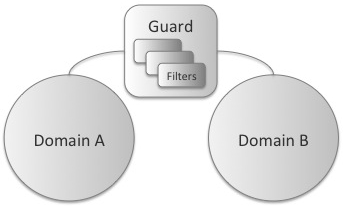
\includegraphics[width=3in]{model-phi-crop}
\caption{Taxonomy ($\phi$)}
\label{fig:model:taxonomy-phi}
\end{figure}

Generally one of the domains supports more sensitive information than the other, but that is not always the case.  In the models we have examined this has certainly been true, but classified information for example  is commonly stored in \textit{compartments} which are separated by clear \textit{need-to-know} policies enforced by access lists and classification guides.  These kinds of compartments contain information at similar levels of classification, but contain distinct informational elements that should not be combined.

In these kinds of systems, specific rules regarding information transfer and domain characterization are tightly bound to individual filter implementations.  They are based on \textit{a priori} knowledge of the domains the guard connects, and therefore are tightly coupled to the domains they connect.  Furthermore, the filter elements are standalone within the system, in this classification, not availing themselves of external resources.  Rather, they examining information transiting through the filter based purely on the content of that information.

\subsection{$\alpha$-level Overlay Systems}
The $\alpha$ overlay classification contains systems that have begun to integrate policy-centric usage management.

Both policies and contexts are dynamically delivered to the system.

The dynamic delivery of context and policies allows these kinds of systems more flexibility with policy evaluation.

The $\alpha$ category begins to integrate policy-centric management rather than using strict content filtering.

\begin{figure}[!t]
\centering
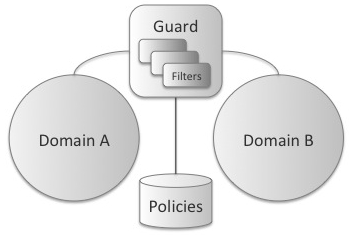
\includegraphics[width=3in]{model-alpha-crop}
\caption{Taxonomy ($\alpha$)}
\label{fig:model:taxonomy-alpha}
\end{figure}

Here, we again have at least two domains, Domain A and Domain B, though we could potentially have more.  $\phi$ type systems require domain specific information to be tightly coupled to the filter implementations.  Separating the permissions, obligations, and other constraints from the filters and incorporating them into a specific separate policy entity frees the Guard from this coupling and provides additional flexibility to the system.

The guard can continue to use filters to process data.  These filters however are now more generic and decoupled from the specific domains it manages.  The choice of using a specific filtering model rather than some other kind of construct is a design detail level to implementers.  That said however, individual filters will be remarkably different and still need to understand the ontologies over which specific licenses are defined.

The policy repository is key to the implementation and differentiation of this taxonomy category.  This repository can be implemented as a separate repository keyed into via a data artifact's unique URI, for example.  It could also represent a policy sent in tandem with a data artifact in a data package.

The policy repository may be implemented as some kind of external service, and as such, represents the first such external service explicitly used in this taxonomy.  Other external services may well exist and be used to adjudicate information transfer decisions as well.

\subsection{$\beta$-level Overlay Systems}
The $\beta$ taxonomic category begins to integrate policy-centric processing with router elements in a given network.  While this work is centered on using overlay technology to illustrate and implement these concepts, it is important to note that this kind of distributed policy-centric processing could very well be distributed into the physical routing fabric of a given network as well by extending Software Defined Networking systems like OpenFlow \cite{proposal:openflow}.

\begin{figure}[!t]
\centering
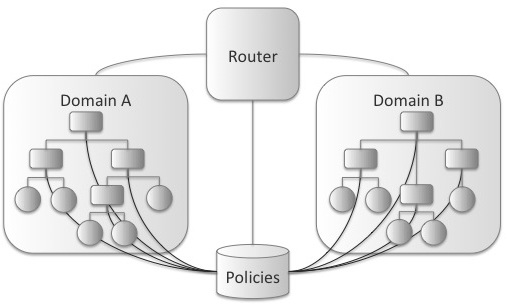
\includegraphics[width=3in]{model-beta-crop}
\caption{Taxonomy ($\beta$)}
\label{fig:model:taxonomy-beta}
\end{figure}

In this model we can also host multiple domains as a result of flexible policy-based content examination.  Each domain hosts a network of some kind, though that hosted network could very well be a degenerate network of a single system.  Each network hosted in a domain is hierarchical, with specific computational nodes embodied by workstations, tablet computers or mobile devices, and routing points embodied by routers or switches of some kind.

Policy evaluation in this model has begun to penetrate into the routing elements of the specific domain networks.  Here, note that we have started to penetrate into the routing fabric of the network by doing content evaluation at router points.  Content-based switching networks have been successful in other domains, and such techniques can be used here to provide policy evaluation capabilities.  

Certain types of traffic are easier to evaluate than others however.  For example, HTTP requests and responses are easier to examine that TCP packets.  When examining TCP packets, systems generally require additional context to select an appropriate packet window (e.g. the number of packets cached for examination).  HTTP traffic does not usually require this kind of flexibility.

This migration of policy evaluation into the routing fabric provides for enhanced data security and better network management, especially if part of a network is compromised.  Now that policy decisions can be made at the router level in a given network, we are starting to have network security in depth rather than simple perimeter protection.  This not only provides the ability for additional information protection, but also allows for different compartments holding information at different need-to-know levels to be created ad-hoc under different routing segments.  In cases of network compromise, this kind of dynamic policy enforcement can also allow for quick node excision as well.

\subsection{$\gamma$-level Overlay Systems}
The $\gamma$ compartment has integrated policy evaluation with compute and routing nodes.  Here, policies can be evaluated against content at all network levels --- nodes emitting requests, nodes fielding requests, and all routing elements in between.

\begin{figure}[!t]
\centering
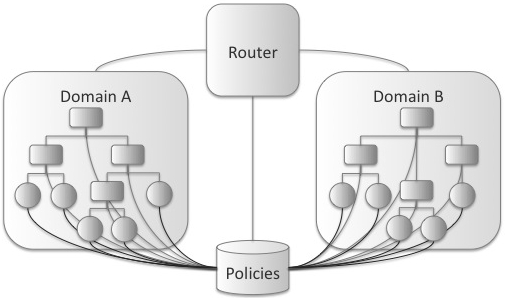
\includegraphics[width=3in]{model-gamma-crop}
\caption{Taxonomy ($\gamma$)}
\label{fig:model:taxonomy-gamma}
\end{figure}

We see that the policy repository is supplying services to all computational elements in both domains.  This gives us increased granularity with respect to data compartmentalization by integrating information security into each network element.  At this point, the network can create compartments of single nodes, while previously in $\beta$ level systems compartments could only be created under specific routing elements.  At this level, we can also provide services revoking data access based on policy evaluation decisions when needed.

Furthermore, individual node exclusion is possible as well. $\beta$ classified systems could excise network elements under specific routers by dynamic policy application.  Now, we can apply the same functionality to individual compute nodes.  For example, if a networked device like a smart phone is compromised, that device can be removed from access quickly or used to feed mis-information to adversaries.

\section{Taxonomic Analysis}
The various levels of the taxonomy vary primarily with respect to the inclusion of policy-based usage management and overlay structure.  $\phi$ type systems are not structured with overlay use in mind, nor do they use policy-centric management.  Conversely, $\gamma$ type systems are both purely policy oriented and completely overlay structured.

As systems move through the various levels of the taxonomy they gradually move from one side of the spectrum to another.  Overlay structures, hierarchical or otherwise, gradually migrate into the network begining with $\beta$ systems.  Policy orientation is injected into the architectures starting with $\alpha$ systems and moving into the network fabric in parallel with overlay inclusion.

\subsection{Policy-centricity}
In these systems policy based management supplies distinct advantages over filter-centric information control.  This kind of policy-centric usage management is more content specific than filters, more flexible, and is more expressive than filter-centric systems.

\subsubsection*{Content Specific}
Filters, in filter-based systems, are not coupled to the content passing through the system.  Rather, they are usually tied to the characteristics of attached networks.  For some filters, that is not problematic.  Malware filters, for example, are very general and do not need to have an understanding of filtered content and are not sensitive to that content at all, though they can be very sensitive to specific context.  This limitation does however prohibit filters from doing anything content specific.  Due to their deployment limitations, in that they are deployed to such a system via a process distinct from processing content, they are unable to use presented content or current dynamic context to influence information processing decisions.

Consider content $c$ impacted by a dynamic context $d$ where $d$ is defined in terms of the content itself, the person or system requesting that content, and the environment in which that request is made.  Here, only under certain specific environmental conditions is that requesting agent allowed access to the requested content.  Ergo, the decision with regard to pass the content to the requester is based upon characteristics of the content related to dynamic changes within the environment.  A filter-centric solution like that contained within the $\phi$ level of the taxonomy is unable to change filter rules based on changes like new content or environmental alteration.  A policy-based system, on the other hand, is able to express the content specific policy easily for more dynamic evaluation.

For example, if $c$ contains information that can only be accessed for a specific time period, a static filter simply cannot determine that the information in $c$ is no longer appropriate for dissemination after that time period ends.  That kind of evaluation requires meta-data associated with $c$ that specifically describes these time bounds and a dynamic contextual evaluator able to determine when that window of access has closed.  That meta-data in this case is a policy.

\subsubsection*{Flexibility}
Policy-centric systems are more flexible than filter-based counterparts.  In a filter-based solution, the type of content that can be evaluated is tightly coupled to the filters installed.  If a given piece of content is new to a given filter-centric solution, that content cannot be appropriately examined and must be submitted for human review.  A policy-based system is designed to be more general.  Based upon a common ontology ~\cite{JaHeLa:10}, the evaluation system can be very general with respect to it's evaluation of a given policy.  A general policy engine can handle a great variety of different content as long as the policies associated with that content correspond to known domain ontologies.  This generality leads to a greater amount of flexibility with respect to what can be expressed in a specific policy, and leads to a more flexible maintainable system.

A filter is going to have a specific responsibility, like redacting sensitive words from a document, for instance.  In order for that filter to redact those sensitive words, it must have access to some kind of list of what those sensitive words are.  Remember, $\phi$ level systems use static filters, so that filter can only be updated when the filter itself is updated.  Now a policy-centric system on the other hand can have a policy associating sensitivity with various areas of content in a specific document.  In this case, all the system must do is understand the sensitivity described in the policy associated with the content, and can then redact that content if needed.  The ontology describing the areas of sensitivity will change more slowly that the possible content itself, leading to a more flexible maintainable system.

This is of course a simple example solvable by creating a dynamic list; the key point of the above example is that the specificity of the filters requires additional complexity in the filter system itself.  The generality of the policy-centric system allows the complexity to be more clearly expressed and contained within the policy file.

\subsubsection*{Expressiveness}
While filters can process content at specific perimeter points, it's lack of reach into a given network fabric limits the power a given filter can actually have over transmitted content.  A policy associated with content, when transmitted with content, can reference much more than the semantics of the protected content.  That policy can describe specifically, in detail, how that content can be used.  Filters simply cannot exercise that level of control.

Assume a distributed system with multiple filter points.  In this kind of system, information distribution can be controlled via deployed filters at a relatively fine level of granularity.  This kind of distribution control cannot influence the use of protected content however --- one that content is distributed, possessors are accorded full access.

Policy enabled systems are not limited in this way.  Policies, when coupled with policy evaluation tools, can exercise control not only over distribution and routing, but also over use of distributed content at endpoints.

These advantages accrue in usage management systems as policy capabilities are propagated through the overlay fabric.  Some of these advantages, like expressiveness, appear simply by beginning to use policies instead of filters.  The remaining two have more of an impact as additional policy-centric nodes combine to form an overlay system suitable for cloud deployment increasing their impact as they move from $\alpha$ to $\delta$ types of systems.

\subsection{Overlay Structure}
Overlay structure integration exhibits clear advantages over single point perimeter systems as well.  Specifically, overlay systems are more partition-able than perimeter solutions, enable content throttling, provide capabilities for dynamic content control, and allow content to be more traceable.

\subsubsection*{Partition-ability}
Administrators typically deploy filter-based perimeter protection at strategic routing points on secure networks.  These kinds of networks are designed with specific regions of enhanced sensitivity separated by cross domain management systems regulating information flows \cite{proposal:nsa-arch,proposal:raytheon-arch,proposal:bah-arch}.  While sensible from the perspective of each protected region as a secure domain, this design thinking begins to fall apart when exposed to the very real threat of the malicious insider.  Boundary-centric information flow control is impossible to realistically achieve when the actual boundaries between malicious actors and system users is constantly in flux.  When a malicious actor can be anywhere within a system, boundaries are simply too dynamic to be realistically recognized.  In order to surmount this fluid system posture, designers must adopt a security in depth mindset.

Application layer overlay networks enable this kind of defense in depth via the possibility of partitioning.  A given overlay system depending on the level of overlay inclusion can partition the user space and by doing so decrease the attack surface available to a malicious insider.  $\phi$ and $\alpha$ level systems based on perimeter filters simply do not present this ability.  Systems beginning with $\beta$ provide the potential to create need-to-know cells of finer granularity up to $\delta$ type systems in which cells can be created at the level of specific content.  These need-to-know cells serve to help quarantine possible intrusion into the sensitive distribution fabric if that fabric is compromised by helping isolate that system failure within the compromised cell.

For example, assume a hypothetical system with nine nodes connected along a single data plane within an prototypical secure network.  With perimeter defenses, if one of those nodes is compromised, a malicious actor can begin to monitor communications traffic between all network nodes, effectively compromising the entire network.  In this same network, if designers partition the system into three overlay cells of three nodes, a similar intrusion in one of those cells will effectively only compromise that cell, leaving the other two cells unaffected.  This decrease in possible targets for compromise effectively decreased the network attack surface from any give node by $\frac{2}{3}$, correspondingly increasing the security posture of the system.

\subsubsection*{Content Throttling}
Perimeter located filter systems only have the opportunity to control sensitive traffic at that initial boundary.  Information located in repositories behind that boundary is not subject to control if it is retrieved by an agent also ensconced behind that same system boundary.  Granted, control can be exerted at the repository level, but in a system with more than one repository, this is if limited impact.

A partitioned cell-oriented system, on the other hand, provides greater opportunity for information monitoring and control.  The partitions applied atop the physical infrastructure provides additional potential control points requests must cross in order to access needed information.  Furthermore, less random cell design provides the capability to unify repositories however needed to provide tight control of information dissemination.

Our hypothetical nine-node system, for example, provides no control over information dispatched from one of the contained nodes to other contained nodes in its initial design form.  There are simply no control points within that nine-node network at which to monitor and control information flow.  Partitioning that space into three three-node cells provides at least two potential control points for inter-cell requests at which information flow can be monitored.  In cases where a malicious insider is actively collecting and hoarding data for exfiltration, these additional control points give system administrators the ability to automatically throttle the rate at which sensitive material can be accessed by users to increase the cost of data collection and increase the likelihood of agent discovery.

\subsubsection*{Dynamic Content Control}
Singular perimeter solutions due to their lack of internal control points also forgo the ability to provide dynamic content control.  Once information has traversed a given perimeter access point, it is no longer under the control of that point and can no longer be retrieved, accessed, monitored, or modified.  Overlay solutions with internal control points can provide the ability to continually monitor and control disseminated information.

Within a given overlay system, depending on that system structure, data can be more rigorously controlled.  $\beta$ and $\gamma$ systems provide the ability to dynamically change information access via contextual changes at a finer grained level than perimeter solutions can.  $\gamma$ systems can in fact provide the ability to retract information access on a per request basis.

This kind of control is especially useful in situations where external partners may temporarily need access to sensitive information for a specific short period of time, say during some kind of joint exercise or activity.  $\gamma$ systems can provide that access only during the window of operation, and retract that access when that window closes.  This kind of use is common in joint military operations with coalition partners, for example.

\subsubsection*{Traceability}
The singular location of perimeter filter solutions also precludes easy information traceability.  Data requests within a given network sans internal controls is more difficult to trace than an overlay solution with a partitioned cell structure that is tailored to the specific information requested (say, XML databases or semantic web content).  The partitioned overlay requires requests to traverse multiple routing nodes at which request and response content can be examined and stored for later analysis and visualization.  Perimeter solutions without this kind of structure simply cannot monitor flows at this finer-grained level.

The strengths of overlay systems over single perimeter points gradually increase as overlay structures increasingly permeate any given system.  Some abilities, like access repudiation, can only occur with smart licensed artifacts at the $\gamma$ level.  Others, like traceability or throttling, become more effective as a system architecture traverses from lower to higher levels of capability within the proposed taxonomy.
\section{Experimental Support}
As we have shown, information-centric networks provide new ways to secure information, but the potential costs are still undefined.  This kind of repeated content analysis, enabled by information-centric computation, can potentially delay information delivery unacceptably.  Information integrity can also be damaged using some possible approaches.  The specific impacts on availability and integrity of these increased confidentiality mechanisms are vital to understand when selecting specific approaches.

For example, removing information from content prior to transmittal over unsecured network paths certainly protects that removed content, but destroys the integrity of the transmitted information.  Likewise, constant encryption and decryption of data to enable repeated examination of transmitted content will certainly have a negative performance impact.  The next two chapters describe exactly how the prototype information network is implemented, and how these approaches impact information confidentiality, integrity, and availability.

\chapter{Experimental Configuration}
A key concept in our current work is the separation of content management from physical communication networks.  In the past, content was controlled via partitioning and physical network access management.  Physical networks were tightly controlled as a way to manage access to sensitive content.  Classified networks in common use today are canonical examples of this kind of approach to content management.  Access to these networks is tightly controlled by classification authorities and the ability to transfer content from these networks to more open systems is rigorously managed.  Corporate systems have also commonly used this kind of approach, though not usually with so much regulation or rigor.

This kind of approach is not scalable however.  It imposes huge costs and infrastructural requirements that are becoming too large to effectively manage.  Furthermore, future systems containing sensitive information require similar security features, and simply cannot be developed without custom controlled infrastructure.  Health care systems, for example, have huge security needs and a more finely grained level of application than even deployed government systems.  These systems will contain exabytes of data, all of which needs to be explicitly controlled, managed, and reviewed by those associated with specific managed records.

\begin{figure*}[!t]
\centering
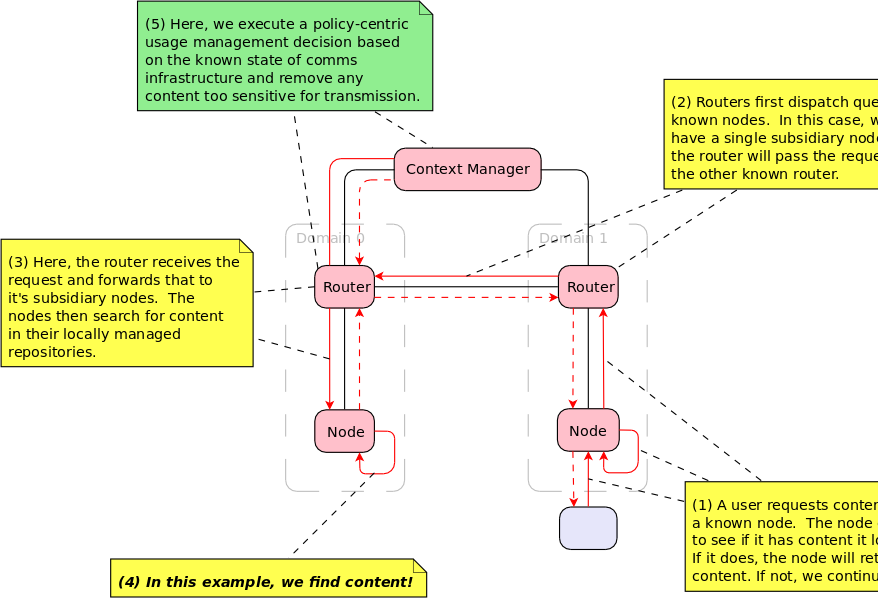
\includegraphics[width=6in]{cross-domain-prototype}
\caption{Simulation Logical Configuration}
\label{fig:model:cross-domain-prototype}
\end{figure*}

\section{Overlay Implementation Concerns}
A key concept in our current work is the separation of content management from physical communication networks.  In the past, content was controlled via partitioning and physical network access management.  Physical networks were tightly controlled as a way to manage access to sensitive content.  Classified networks in common use today are canonical examples of this kind of approach to content management.  Access to these networks is tightly controlled by classification authorities and the ability to transfer content from these networks to more open systems is rigorously managed.  Corporate systems have also commonly used this kind of approach, though not usually with so much regulation or rigor.

This kind of approach is not scalable however.  It imposes huge costs and infrastructural requirements that are becoming too large to effectively manage.  Furthermore, future systems containing sensitive information require similar security features, and simply cannot be developed without custom controlled infrastructure.  Health care systems, for example, have huge security needs and a more finely grained level of application than even deployed government systems.  These systems will contain exabytes of data, all of which needs to be explicitly controlled, managed, and reviewed by those associated with specific managed records.

Separating content networks from physical networks enables network infrastructure virtualization and multi-tenancy.  Use the popular file-sharing system BitTorrent as an example.  BitTorrent is a content network optimized for download efficiency.  It run over traditional TCP/IP networks, but manages traffic according to specialized algorithms unique to BitTorrent.  These algorithms take advantage of the asymmetry between upload and download speeds of typical home-use Internet systems in which upload speeds are regularly an order of magnitude slower than download speeds.  By partitioning content into distinct sections and downloading them from multiple clients, a downloading node can effectively use all available download bandwidth and is no longer necessarily constrained by the upload bandwidth of a serving peer system.  We use a similar approach, in that our hypothesized systems also overlay TCP/IP traffic, but rather than optimizing download speeds we focus on content usage management.

Just as systems like BitTorrent runs over current established protocols, usage management overlay systems could as well.  They support multi-tenant cloud computing systems by providing secure compartmentalized access to managed information.  They also support the ability to create and use integrated overlay systems between multiple cloud providers, supporting running of overlay components in systems hosted at Amazon while accessing nodes executing on Rackspace infrastructure.

Content networks must deal with situations analogous to those encountered in previous physical systems.  Specific examples include cross-domain monitoring and content mashing.  Both problems are currently areas of active research within physical networks and need extensive examination in overlay systems as well.

To begin with, in content-specific overlay networks, cross-domain routing can become an even more pervasive issue.  Currently, cross-domain data processing guards are installed on the perimeter of sensitive networks where they can monitor and manage outgoing and incoming traffic.  In content networks, these kinds of systems can begin to multiply within the information transmission fabric.  In physical networks, the network topology is fixed and is established when the network is installed.  After installation, changes in the essential network topology are cost-prohibitive and correspondingly rare.  Overlay systems do not suffer from this high cost of change, and can easily morph from one topology to another.  As additional content enclaves appear within a given overlay topology, the need for content usage management between those enclaves increases.

Mashup scenarios become similarly common.  As additional sources of accessible data appear, opportunities for inappropriate data combinations increase at best geometrically.  Data combinations need to be likewise managed to prevent inappropriate data combinations.

\section{Implementation}
Our current completed prototype shows that overlay routers can in fact use licenses bundled alongside content to modify transmitted content based on dynamic network conditions.  Running on a single host over HTTP, it simulates two content domains and communication between them.  The communication link has uncertain security state and changes over time.  Note that it currently runs on a single host with varying ports, but it could easily run on multiple hosts as well.  The current single host configuration is simply to simplify system startup and shutdown.

License bundles are hosted on the filesystem, though they could be hosted in any other data store.  These artifacts are currently XML.  They are stored in a directory, and the license file has a LIC extention while the content file has an XML extension.  Both the content and the license files have the name of the directory in which they reside (for example, if the directory is named test, the license file is named test.lic and the content file test.xml).  In this context, the directory is the content bundle.  The license and content files are simply documents and port to document-centric storage systems like MongoDB easily.  They can certainly be stored in traditional relational databases as well.

The system itself has two domains, Domain 0 and Domain 1.  Each domain consists of a client node and a content router node.  Requests are initially served to client nodes.  If client nodes do not contain the requested content, they the forward that request to their affiliated content router.  The content router will send that request to all the content routers of which it is aware.  Those other routers will then query associated client nodes for content.  If the requested content is in fact found, it will be returned to the original requesting router and then to the requesting node.  If the content is not found, HTTP status 404 codes are returned to requesting routers and nodes.

All router-to-router content traffic is modified based on security conditions.  A Context Manager maintains metadata regarding network paths.  If a given network path is only cleared for data of a certain sensitivity level, a transmitting router will remove all license information and content that is associated with higher sensitivities, and then transmit only information at an appropriate sensitivity level over the link.

Figure \ref{fig:model:cross-domain-prototype} shows the prototypical workflow through the system across the domains, and Figure \ref{fig:model:prototype-physical-config} shows the current system configuration of the simulation, with the cross-domain link highlighted in red.  The system is current configured to use ports 4567 through 4571.

All content requests are via HTTP GET.  Link status can be changed via HTTP POST and we use the CURL command to exercise the network.

This proof-of-concept does implement a simple overlay network for usage managed content over HTTP, easily extensible to HTTPS.  Changes in the context of the network dynamically change the format of transmitted content.  All source code for this simulation is publically available on GitHub, at https://github.com/cclamb/overlay-network, with documentation on how to run the simulation.

\begin{figure}[!t]
\centering
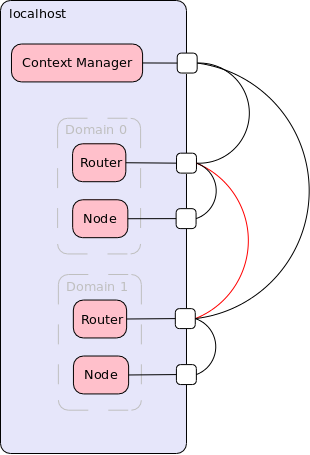
\includegraphics[width=3in]{prototype-physical-config}
\caption{Physical Simulation Configuration}
\label{fig:model:prototype-physical-config}
\end{figure}
\section{Using the Network}
This system is now defined, with primary interface and data type definitions, and implemented.  At this point, it can filter information through defined nodes implementing different strategies in accordance with specific defined rules.  It is also instrumented so that it can generate accurate timing information needed to measure availability impacts of confidentiality strategies on tranmitted information.  The next chapter will cover specifically how these results were collected, the results themselves, and interpretation of what those results imply.

\chapter{Experimental Results and Conclusions}
Experiments using this inter-cloud framework yield promising support for this approach.  They show only a slight degradation of information availability as a result of this network permeated security approach, with redaction and encryption demonstrating the smallest degradation at a higher impact on delivered information integrity.  Rerouting-based approaches have the most performance degradation. Encryption generally has the smallest impact on information integrity.  This is most evident when network effects are removed from evaluation.  Non-hierarchical and hierarchical networks have very similar performance with respect to content availability as well.

The goal of this experimental work was to characterize confidentiality, integrity, and availability impacts of these information-centric network security approaches in both hierarchical and non-hierarchical configurations.  The specific strategies addressed were redaction, rerouting, and protection (via encryption), and these strategies were evaluated from the perspective of confidentiality, integrity, and availability over hierarchical and non-hierarchical networks, and on standalone nodes. Confidentiality was measured via the control used to protect information.  Removing information entirely provided the highest measure of protection but is akin to unplugging a computer to improve its cyber-security posture.   Routing information through a more secure channel is the next most powerful approach, followed by sensitive information protection via strong encryption.  A 256-bit AES-CBC encryption scheme was used in this work.  Availability was measured by the delivery of information and the time required to ensure information delivery, measured by end-to-end network performance.  Integrity is a function of the alterations to the information required for secure delivery in the tested scenario.  Unaltered information has the highest integrity, followed by information that is still complete but protected via encryption, information that has been divided and rerouted, and finally information that has had content redacted.  Though combinations of strategies in a given network can be specified, as strategies are specified by network node, in these experiments only a single strategy in each network was used to more clearly attribute strategy performance impacts. Identical policies were used in each simulation to ensure the same amount of required usage management actions, limiting the effects on availability to the approach rather than differing policy.  In each case, a control simulation that did not incorporate any usage management was run to provide a performance baseline.  

\section{Hierarchical Networks}
In these tests, a simulated $\gamma$-categorized system was examined.  This is the kind of system that organizations like the UCDMO have identified as the final goal state of their work, systems that incorporate policy-centric management in the fabric of systems and networks (12).  The kind of components required to do this kind of policy-based content-sensitive evaluation do not currently exist, and components of these kinds of systems are only now beginning to emerge.  Systems like OpenFlow, when they have stronger hardware support, can begin to provide some of these kinds of capabilities.  OpenFlow enabled systems are not yet common or widely used however, and though they do provide the needed control for these kinds of systems, the do not supply the necessary policy interpretation and evaluation.  As a result, this experimental work was conducted over an HTTP overlay network, at the application layer.  Using a document-focused protocol makes content evaluation simpler as well, as systems can evaluate all content when it transits a network rather than maintaining a buffer of content required when processing packet-level communications.

In order to develop a stronger perspective on the network performance, delivery times were measured from three separate nodes.   One node is hosted in Comcast's infrastructure (a large local internet service provider), one at Amazon, and another at Rackspace.  The tested network had four levels.  The first level had a single router node.  The next level had two routers, both connected to the router in the first level.  The third level contained four routers, two attached to each of the routers at the level just above.  Finally, the fourth level contained nodes, distributed so that two level three routers had three nodes, one level three router had two nodes, and the last level three router had four nodes.  The first three levels were essentially a binary tree.  The network was queried from five different locations.  The node that contains the content was queried directly (the home node).  A node under the same router as the home node was then queried for content (the peer node).  Next, queries were sent to a node under a different router, but connected to the same second level router (the neighbor node).  Finally, two nodes on the other side of the network were queried for content (the distant (1) and (2) nodes).  Each node was queried for content 50 times in each simulation, for a total of 250 queries per simulation.

\begin{figure}[!t]
\centering
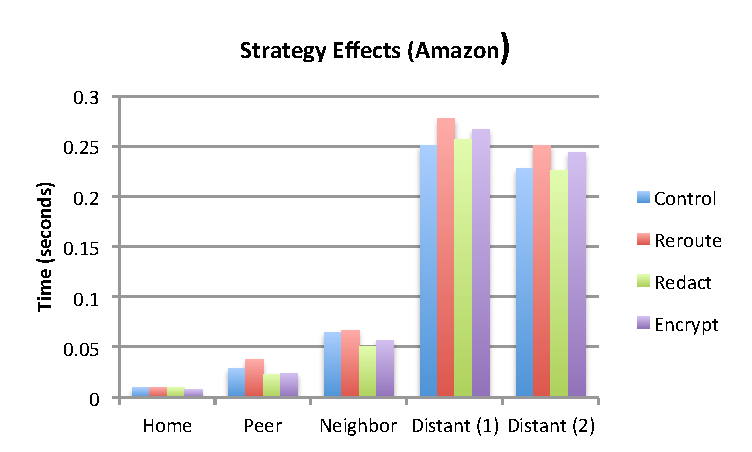
\includegraphics[width=6in]{strategy_effects_az}
\caption{Hierarchical Results from Amazon}
\label{fig:model:amazon-results}
\end{figure}

Figure ~\ref{fig:model:amazon-results} shows performance results from the Amazon testing node.  The access times for the content from the home, peer, and neighbor nodes were by far the smallest.  As the testing node was hosted in the same datacenter as these three nodes, that was to be expected.  The access times for both distant nodes was, however, surprisingly high.  With that in mind, the overall trend for response times is sensible however, with access time increasing as the requesting node is farther away from the content in the information network.  Queries from distant nodes need to traverse five information routers, while home, peer, and neighbor nodes only traverse one, two and three, respectively.  Also surprising was the finding that rerouting was generally more expensive from an availability perspective than encryption-based approaches.  This is likely attributable to the costs associated with attaching to the external SMTP server, hosted at Google, used as the out-of-band communications channel.  Also evident is remarkable performance variability.  Control data was collected at different times than experimental data, and infrastructural demands seem to have driven the control data availability to be less than that of other, managed approaches.  Overall, this evidence of variable performance due to external provider demands leads to the conclusion that overall, the availability costs of the various approaches are in fact negligible.

\begin{figure}[!t]
\centering
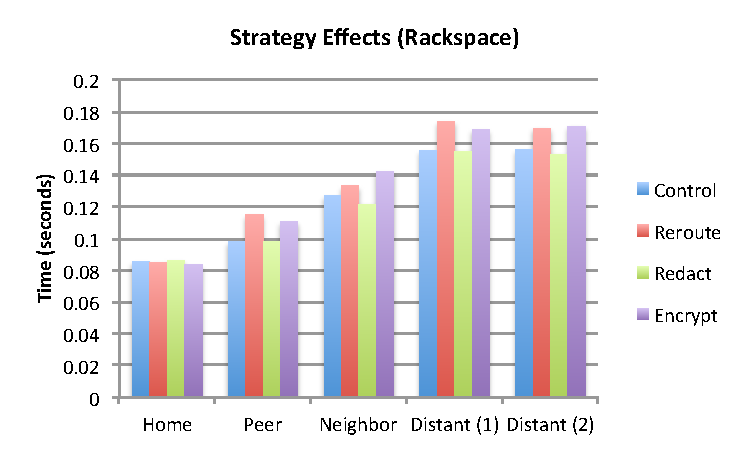
\includegraphics[width=6in]{strategy_effects_rs}
\caption{Hierarchical Results from Rackspace}
\label{fig:model:rackspace-results}
\end{figure}

Figure ~\ref{fig:model:rackspace-results} shows similar results to Figure ~\ref{fig:model:amazon-results}.  Here, the query times are much higher for the home and peer nodes, but actually lower for the distant nodes.  In this case, the content is still hosted in Amazon's infrastructure, but the testing node is at Rackspace.  As a result, the longer response time for content from the home node is to be expected.  Queries to distant nodes are actually shorter than the previous calls into distant nodes from Amazon.  This stems from the fact that the distant nodes are both hosted at Rackspace.  This locality shortens the round trip distance for a request.  Previously, from Amazon, a content request would need to travel from Amazon's east coast data centers to the Rackspace data center in Dallas, then back to the east coast for content, then back to Dallas, then back to the east coast.  In this test, the request only travels from Dallas to the east cost, and back.  Nevertheless, the overall performance profile is sensible, reflecting the expected shorter latency between home, peer, and neighbor nodes when compared to distant nodes.  Similar to amazon, cases when the control latency is higher than experimental latency emerge, indicating some amount of infrastructure performance variability.  In Figure ~\ref{fig:model:rackspace-results} however, it is evident that overall encryption and rerouting impact performance more than redacting, as would be expected.  Rerouting again has high overall impact, likely as a result of contacting Google's remote SMTP services.

Figure ~\ref{fig:model:comcast-results} Shows performance results measured from Comcast.  Interestingly, they show significant variability when accessing nodes hosted at Amazon, and more predictable performance when accessing nodes in Rackspace's infrastructure.  The overall variability does not follow the expected pattern of shorter response times when accessing content from nodes close to that content, except in a few cases.  This illustrates the kind of performance variability one can expect from an external service provider.

Integrity impacts are the result of approach rather than platform.  Redacting content destroys information integrity, as information is removed and not delivered to requesters.  Encryption maintains integrity the best of the three alternatives as information, even though encrypted, is still delivered, and delivered in the context of the query response at that.  Rerouting is better than redaction, in that sensitive information is still delivered, but worse than encryption, as it is not delivered within the response context and is sent out-of-band. Simulations removed sensitive information from the information network and dispatched it to a user's email address via SMTP over TLS when the selected strategy was rerouting.  This impacts information availability, as email delivery times can be highly variable.  In these experiments, delivery could take anything from a few seconds to a few minutes.

\begin{figure}[!t]
\centering
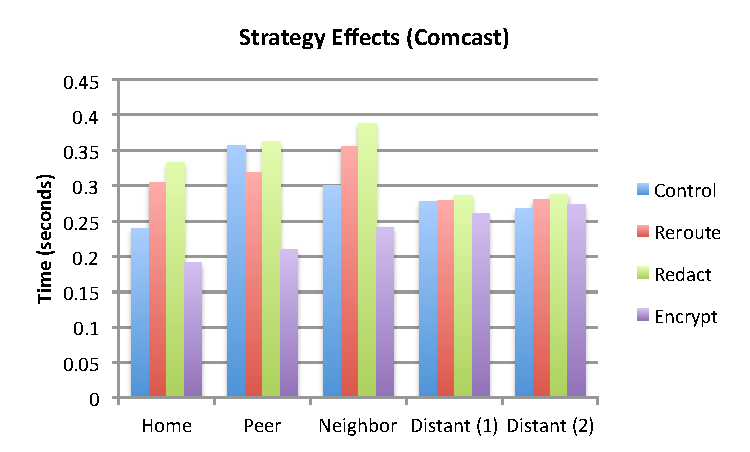
\includegraphics[width=6in]{strategy_effects_local}
\caption{Hierarchical Results from Comcast}
\label{fig:model:comcast-results}
\end{figure}

Confidentiality is likewise impacted primarily by approach and not by infrastructure.  Redacting sensitive content provides the best confidentiality protection, as sensitive content is simply not exposed.  Encryption is likely the worst solution from a confidentiality perspective as content encryption is a delaying tactic against a determined, well-resourced adversary.  Rerouting may be better or worse than encryption as an approach, depending on the confidentiality of the out-of-band channel.  If the security of that channel can be guaranteed, then it is likely a better approach.  If, on the other hand, the security of that channel is more variable or difficult to ascertain, encryption may be a more reliable approach.

Overall, results show that, from a performance perspective, the rerouting approach fares the worst, but only slightly, and certainly not in all cases.  Both results from Amazon and Rackspace, in Figures ~\ref{fig:model:amazon-results} and ~\ref{fig:model:rackspace-results}, show encryption as generally taking the second largest performance hit, just following rerouting.  Furthermore, network effects have a much larger impact on performance than information protection approaches.  The query to the home node is an excellent predictor of overall network stability, as content delivered directly from a home node is only subjected to the selected information protection strategy once.  Note that when queried from Amazon or Rackspace, the home node timing results are very close to uniform.  Queries from Comcast, however, are much more varied, indicating more highly variable quality of service within the Comcast network.  This is also supported by the gross distribution of response times.  Within both the Amazon and Rackspace networks, the farther a queried node is from the content requested, the worse the latency, as expected.  Comcast's network has a much more uniform information network response time overall as the processing time of the information network simulation is overshadowed by the highly varied performance of Comcast's physical network.  Availability is surprisingly uniform across all confidentiality strategies, showing little impact on end-to-end processing times.

\section{Non-Hierarchical Networks}
In order to test non-hierarchical networks, a simple branching network of participants was used, identical in form to the hierarchical network, though queries could be routed through the network from any point.  Queries could come into any node on the network, and would propagate through the network to the requested content, evaluating the returned content as it passes back through the network in response to the initial query.

In these experiments, the node that contains the content was queried, then the node immediately next to that content node, and so on, to a distance of five nodes.  The home node again contains content, and the additional nodes are marked by the distance in node count from the home node, starting with Neighbor (1), proceeding through Neighbor (5).  The non-hierarchical network was queried from Rackspace, Amazon, and Comcast, for a total of 250 queries per test, testing the system once per each confidentiality strategy.

\begin{figure}[!t]
\centering
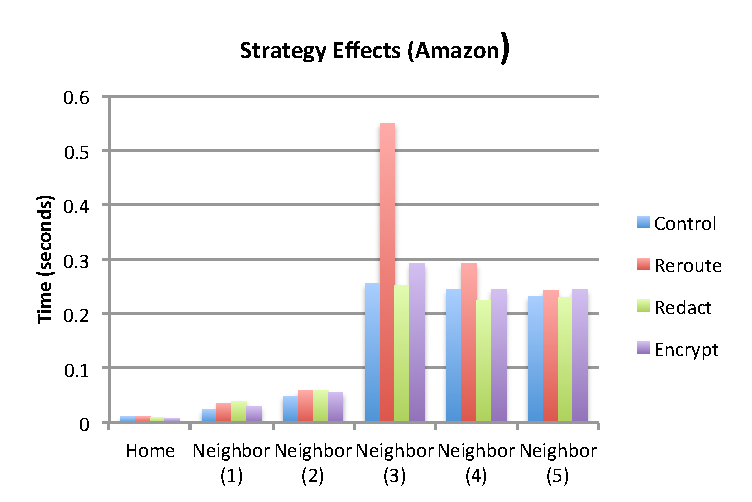
\includegraphics[width=6in]{nh_strategy_effects_az}
\caption{Non-Hierarchical Results from Amazon}
\label{fig:model:nh-amazon-results}
\end{figure}

Figure ~\ref{fig:model:nh-amazon-results} shows the performance of a non-hierarchical network as tested from the Amazon test node.  The content response latency is characteristic of moving farther from the source node through the network.  The request nodes switch from Amazon infrastructure to Rackspace infrastructure starting with Neighbor (3), and this is reflected in the sudden increase in latency.  As the tests originate from Amazon, at the Neighbor (3) node, a request and it's response must travel from Virginia to Texas, then back to Virginia, then back to Texas, then back to the original requester in Virginia.  The spike in latency at Neighbor (3) when re-routing traffic is caused by SMTP delays with systems hosted at Google.  Overall, the distribution is very similar to the hierarchical case.  Also evident is a continuation of the previous pattern in which re-routing is the least efficient strategy, followed by encryption, then redaction.

\begin{figure}[!t]
\centering
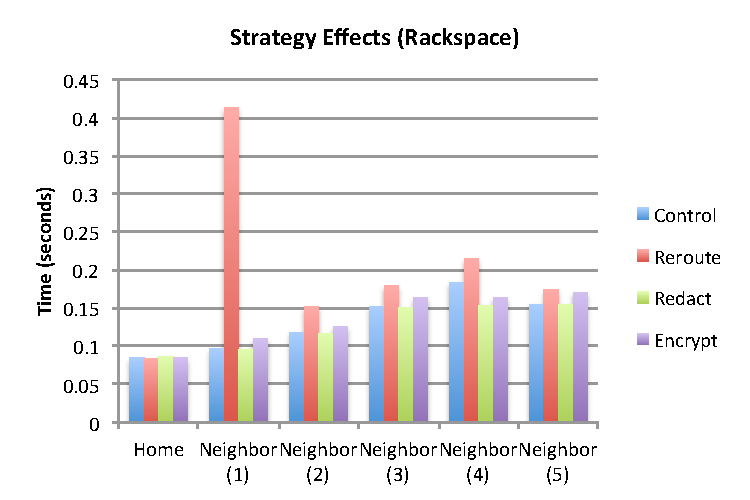
\includegraphics[width=6in]{nh_strategy_effects_rs}
\caption{Non-Hierarchical  Results from Rackspace}
\label{fig:model:nh-rackspace-results}
\end{figure}

Unlike the previous Amazon-based tests, the Rackspace tests shown in Figure ~\ref{fig:model:nh-rackspace-results} latencies seem much more uniform.  This again stems from the fact that each content query will always traverse the distance between Amazon and Rackspace data centers at least once.  Other than that, the distribution again shows an increase in measured latency as the queried node moves farther and farther away from the home node.  Once again, a dramatic spike in latency emerges based on SMTP delays when re-routing information.  The pattern of re-routing having the highest latency continues here as well.

\begin{figure}[!t]
\centering
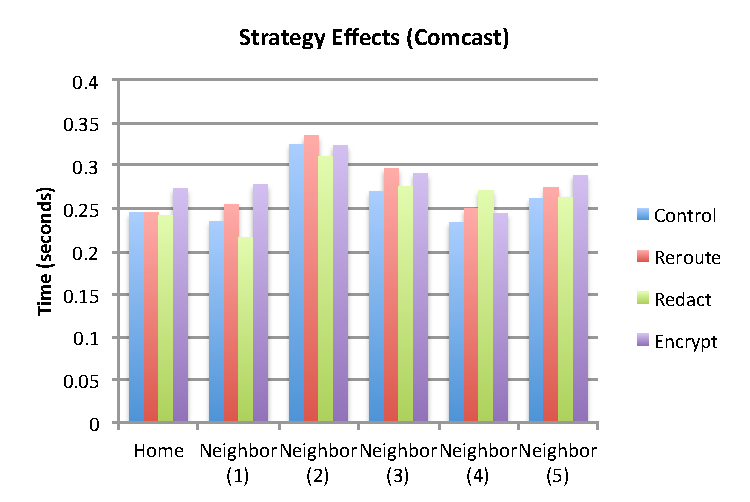
\includegraphics[width=6in]{nh_strategy_effects_local}
\caption{Non-Hierarchical Results from Comcast}
\label{fig:model:nh-comcast-results}
\end{figure}

Results from Comcast, included in Figure ~\ref{fig:model:nh-comcast-results}, shows a fairly regular distribution of response latencies overall.  In this case, the test node is ensconced within Comcast's network infrastructure.  Generally, re-routing is the least efficient approach, but not uniformly.  In this case, network effects created by the physical location of the testing node dominate these results.

Non-hierarchical networks behave very similarly to hierarchical networks.  This is not surprising --- although the nodes are more functionally complex, performing routing and repository functions, once the content is found and delivered the roles the nodes fall into mirror those in a hierarchical network.  For example, in a typical query, a node will receive a request, check the repository for the requested content, and if the content does not exist, pass the request onto the next known nodes.  This does differ slightly from the hierarchical case in that the nodes check for content at each routing step, though this is a very fast and simple test.  Once content is found, the response is routed back the the requester without any repository checks, just as it would be in a hierarchical system.

\section{Removing Network Effects}
Having established the parameters under which confidentiality strategies may be chosen, the next immediate area of concern involves the number of filtering events that can occur prior to a given information network suffering from degraded performance.  Previous results demonstrated that some kind of degradation of performance in the selected network based on distance from content does exist, but that can also be attributed to the distributed nature of the network itself.  Processing performance of a given node must be evaluated free of network effects in order to more clearly understand the availability implications of content filtering itself.

A single node, configured on one of the test nodes in either infrastructure, would yield the type of network effect free performance limits needed.  A node in Amazon's environments was configured such that requests were made of the home node itself, under each of the three confidentiality strategies.  Requests were also directed to the home node without any usage management systems engaged in order to collect control data.  After that initial request, the node was configured with various usage management strategies in order to measure their availability impact.

\begin{figure}[!t]
\centering
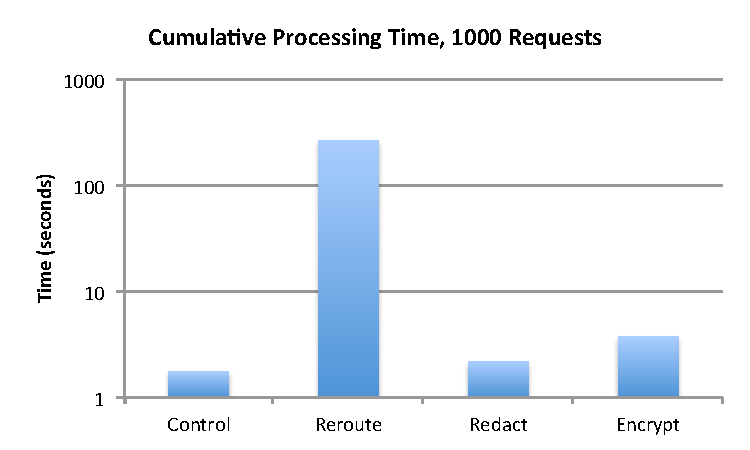
\includegraphics[width=6in]{single-node-results}
\caption{Results from Requests to a Singe Node}
\label{fig:model:single-node-results}
\end{figure}

As shown in Figure ~\ref{fig:model:single-node-results}, with information network effects removed, redaction and encryption have very similar performance overall.  Redaction, as a strategy, is very simple programmatically, and as symmetric encryption is used for information protection, ciphering and deciphering operations are very fast.  Rerouting, in this case, is clearly the worst strategy.  This is a result of the dependency of this strategy on external systems and system configuration times.  Specifically, configuring and using SMTP for each rerouting operation is prohibitively expensive.
\section{Conclusions}
The work described in this paper presents bounds under which to select specific confidentiality strategies for protecting information in content networks.  We first described the state of the art of this kind of information protection in content networks, and introduced the current accepted protection architectures sponsored by the UCDMO.  We then presented a related taxonomy of increasing information protection, describing their advantages and disadvantages and how they could be implemented.  Next, we described our current customizable experimental framework for evaluating various confidentiality strategies.  We closed with a description of and the motivation for our experiments over these networks, the results of these experiments, and analysis of those results.  All simulation code is freely available via Github.

	Overall, confidentiality strategy had little impact on information availability.  Redaction, rerouting, and encryption all performed within similar bounds.  Of these three approaches, redaction damaged information integrity the most, followed by rerouting, and then encryption, depending on the security of rerouting infrastructure.  Redaction provided the most confidentiality, followed by rerouting, and then by encryption (as encrypted content is generally at best a delaying tactic given enough time for cryptanalysis).  Based on these results, rerouting is likely the best general solution, depending on the existence of a secondary secure channel.  Less sensitive information can still be delivered via encryption, especially if that information is only sensitive within a given time window.  Very sensitive information can be redacted, but due to the related damage to integrity, this is only an attractive option when confidentiality is of the utmost importance.
	
	At this point, our information network implementation has integrated three different configurable strategies for information protection, and routes information via an overlay network using HTTP.  Longer term, this project will expand to both incorporate public-key encryption protocols and software defined networking (SDN) capabilities to provide physical control of information routing.  We intend to provide public-key encryption capabilities via an integrated public key infrastructure providing additional privacy and non-repudiation abilities for the network and SDN capabilities via integration with OpenFlow.  Shorter term goals include inclusion of different modes of operation, so that the network can support both request/response and publish/subscribe modes of operation, and more robust development so the system can run as a commercial grade security-on-demand service.


\pagebreak

\bibliographystyle{plain}
\bibliography{bib/proposal,bib/drm,bib/info-centric,bib/rfc}

\end{document}